%%%%%%%%%%%%%%%%%%%%%%%%%%%%%%%%%%%%%%%%%%%%%%%%%%%%%%%%%%%%%%%%%%%%%%%%%%%%%%%
%% LaTeX-Vorlage für Abschlussarbeiten                                       %%
%% (TH Köln -Campus Gummersbach, Fak. 10)                                    %%
%%                                                                           %%
%% Gemäß dem Merkblatt zur Anfertigung von Projekt-, Bachelor-, Master- und  %%
%% Diplomarbeiten der Fakultät 10 von Frau Prof. Dr. Halfmann &              %%
%% Herr Prof. Dr. Rühmann (Version vom 27.01.2008)                           %%
%%                                                                           %%                                                                            
%% Bitte sprechen Sie unbedingt mit Ihrer Betreuerin bzw. Ihrem Betreuer     %%
%% bezüglich der Ausgestaltung Ihrer Arbeit!                                 %%
%%                                                                           %%
%%                                                                           %%
%% MERKKASTEN IN DIESER VORLAGE:                                             %%
%% In dieser Vorlage finden Sie Merkkasten, die Ihnen Informationen          %%
%% zu bestimmten, formalen Aspekten geben. Sprechen Sie immer auch mit       %% 
%% Ihrer Betreuerin bzw. Ihrem Betreuer dazu an.                             %%                       
%% Für die eigene Verwendung der Vorlage entfernen oder kommentieren Sie die %%
%% Merkkasten. Die betreffenden Bereiche für die Merkkasten in der Vorlage   %%
%% sind wie folgt kommentiert: <MERKKASTEN> ... </MERKKASTEN>.               %%                            %%                                                                           %%
%%                                                                           %%
%% LIZENZ:                                                                   %%
%% Diese Vorlage darf nicht kommerziell verbreitet                           %%
%% werden. Eine nicht-kommerzielle Weitergabe ist                            %% 
%% gestattet.                                                                %%
%%                                                                           %%
%% Von Ludger Schönfeld, M. Sc.,
%% 2014-2017                            %%
%%%%%%%%%%%%%%%%%%%%%%%%%%%%%%%%%%%%%%%%%%%%%%%%%%%%%%%%%%%%%%%%%%%%%%%%%%%%%%%

%%%%%%%%%%%%%%%%%%%%%%%%%%%%%%%%%%%%%%%%%%%%%
%% HEADER                                  %%
%%%%%%%%%%%%%%%%%%%%%%%%%%%%%%%%%%%%%%%%%%%%%
\documentclass[a4paper,12pt,oneside]{article}
% Optionen:
% - a4paper => DIN A4-Format
% - 12pt    => Schriftgröße (weitere  
%              grundlegende Fontgrößen: 10pt, 11pt)
% - oneside => Einseitiger Druck

%% Verwendete Pakete:
\usepackage[ngerman]{babel} % für die deutsche Sprache
\usepackage{caption} % Für schönere Bildunterschriften
\usepackage[T1]{fontenc} % Schriftkodierung (Für Sonderzeichen u.a.)
\usepackage[utf8]{inputenc} % Für die direkte Eingabe von Umlauten im Editor u.a.
\usepackage{fancyhdr} % Für Kopf- und Fußzeilen
\usepackage{lscape} % Für Querformat

%% Schriften (Beispiele)
%% Weitere LaTeX-Schriften im "LaTeX Font Catalogue"
%% unter: http://www.tug.dk/FontCatalogue/.
%% ACHTUNG: Ggf. müssen Schriften noch installiert 
%% werden!

% Serifen-Schriften:
\usepackage{lmodern} % Schriftart "Latin Modern"
%\usepackage{garamond} % Schriftart "Garamond"

%Sans Serif-Schriften:
%\usepackage[scaled]{uarial}
%\usepackage[scaled]{helvet}
%%--------------
\usepackage[normalem]{ulem} % Für das Unterstreichen von Text z.B. mit \uline{}
\usepackage[left=3cm,right=2cm,top=1.5cm,bottom=1cm,
textheight=245mm,textwidth=160mm,includeheadfoot,headsep=1cm,
footskip=1cm,headheight=14.599pt]{geometry} % Einrichtung der Seite 

\usepackage{graphicx} % Zum Laden von Graphiken
% INFO: Graphiken einbinden
%
% \includegraphics[scale=1.00]{dateiname}
%
% => Ausgabeformat: PDF-Dokument:
%    Es können die folgenden (Graphik-)formate eingebunden
%    werden: .jpg, .png, .pdf, .mps
% 
% => Ausgabeformat: DVI/PS:
%    Folgende (Graphik-)formate werden unterstützt:
%    .eps, .ps, .bmp, .pict, .pntg
\usepackage{epstopdf}

% Pakete für Tabellen
\usepackage{tabularx} % Einfache Tabellen
\usepackage{longtable} % Tabellen als Gleitobjekte (für die Aufteilung bei langen 
 %Tabellen über mehrere Seiten)
\usepackage{multirow} % Für das Verbinden von Zeilen innerhalb einer Tabelle mit
 % \multirow{anzahl}{*}{Text}

% (Zusatz-)Pakete für Formeln
\usepackage{amsmath}
\usepackage{amsthm}
\usepackage{amsfonts}

\usepackage{setspace} % Paket zum Setzen des Zeilenabstandes
% INFO: Zeilenabstand setzen:
%
% Befehle:
% - \singlespacing  => 1-zeilig (Standard)
% - \onehalfspacing => 1,5-zeilig
% - \doublespacing  => 2-zeilig 
\onehalfspacing % Zeilenabstand auf 1,5-zeilig setzen

% Farbboxen (für die Merkkästen in dieser Vorlage):
\usepackage{tcolorbox}
\tcbset{colback=white,colframe=orange,
        fonttitle=\bfseries}
        
\usepackage{subfigure} 

\usepackage[colorlinks,pdfpagelabels,pdfstartview=FitH,
bookmarksopen=true,bookmarksnumbered=true,linkcolor=black,
plainpages=false,hypertexnames=false,citecolor=black]{hyperref} % Für Verlinkungen
% INFO: Verlinkungen mit dem hyperref-Paket:
%
% Die Angabe von URLs mit dem Befehl \url{} erlaubt einen
% gesonderten Umgang mit Weblinks. Denn die Links werden verlinkt.
% Auch erfolgt automatisch am Zeilenende ein Umbruch des Links.
% Es ist auch nicht erforderlich, Sonderzeichen in der URL manuell zu 
% entschärfen.
%
% TIPP: Sollte ein Umbuch bei einem Link nicht automatisch erfolgen, so kann
% das daran liegen, dass ein/mehrere Zeichen zusätzlich angegeben werden müssen,
% an dem der Link umbrochen werden kann.
% Dies kann mit folgendem Befehl erfolgen (Beispiel):
% \renewcommand*\UrlBreaks{\do-\do_}

% Das Paket "biblatex" für autom. 
% Literaturverzeichnisse:
\usepackage{csquotes} % Für sprachangepasste Anführungszeichen
\usepackage[backend=bibtex,style=alphabetic]{biblatex}
\addbibresource{literatur.bib}           

%%%%%%%%%%%%%%%%%%%%%%%%%%%%%%%%%%%%%%%%%%%%%
%% DOKUMENT                                %%
%%%%%%%%%%%%%%%%%%%%%%%%%%%%%%%%%%%%%%%%%%%%%
\begin{document}
  
  % Deckblatt
  \pagestyle{empty}
  \begin{titlepage}
    
\includegraphics[scale=1.00]{Sources/logo_TH-Koeln_CMYK_22pt}\\
    \begin{center}
      \Large
      Technische Hochschule Köln\\
      Fakultät für Informatik und Ingenieurwissenschaften\\
      \hrule\par\rule{0pt}{2cm} % Horizontale Trennlinie  mit 2 cm Abtand nach unten erzeugen
      \LARGE
      \textsc{Praxisprojekt WS18/19 - Dokumentation}\\
      \vspace{1cm} % Vertikaler Abstand von 1cm erzeugen
      \huge
      Entwicklung einer Objekterkennung für Regal-Systeme,
      mit Hilfe von Bildverarbeitung, in einem Neuronalen Netz\\
      \vspace{1 cm}
      \large
      Vorgelegt an der TH Köln\\
      Campus Gummersbach\\
      im Studiengang\\
      Medieninformatik\\ 
      \vspace{1.0cm}
      ausgearbeitet von:\\
      \textsc{Torben Krause}\\
      (Matrikelnummer: 11106885)\\
      \vspace{1.5cm}
      \begin{tabular}{ll} % Einfache Tabelle ohne Rahmen, mit 2 Spalten erzeugen
          \textbf{Prüfer:} & Prof. Dr. Martin Eisemann \\
      \end{tabular}
      \vspace{1.5cm}
      \\Gummersbach, 28.12.2018
    \end{center}    
  \end{titlepage}
  
  \newpage
  
  % Inhaltsverzeichnis
  \tableofcontents
  \newpage
  \listoffigures
 
  
  \newpage
  \pagestyle{plain}
  \pagenumbering{arabic}
  \setcounter{page}{1}
   
  
  \section{Motivation}
Das richtige Verwalten von Lebensmitteln, welche gekühlt im Kühlschrank aufbewahrt werden müssen, ist nicht immer leicht. Oft müssen schlecht gewordene Lebensmittel weggeschmissen werden, weil sie vergessen werden oder es fehlen Lebensmittel, welche gebraucht werden. Gerade in Haushalten mit mehreren Personen, wie zum Beispiel Familien oder Wohngemeinschaften, ist das Kühlschrankmanagement schwierig, da nicht jeder Bewohner weiß, welche Lebensmittel aus dem Kühlschrank genommen wurden und welche hineingelegt werden. Der häufigste Grund ist dabei die unzureichende Kommunikation unter den Bewohnern. Aus diesem Grund werden schnell verderbende Lebensmittel leicht vergessen oder Produkte durch fehlerhafte Absprache mehrfach oder nicht gekauft. \\ Eine Idee um dieses Problem zu lösen ist den Kühlschrankinhalt mithilfe einer Kamera, welche im Inneren des Kühlschranks angebracht ist, aufzuzeichnen und die enthaltenden Lebensmittel mit einem neuronalen Netz zu klassifizieren. Aus den Ergebnissen der Analyse wird nun eine Produktliste vom Inneren des Kühlschranks erstellt und anschließend in einer Datenbank gespeichert. Über eine mobile Anwendung können die erhobenen Daten dem Benutzer zur Verfügung gestellt werden.
  
  \subsection{Zielsetzung} 
Ziel dieses Projektes ist die Entwicklung eines künstlichen neuronalen Netzes, welches mehrere vordefinierte Klassen zuverlässig erkennt und zuordnen kann. Das Netz soll außerdem so konzipiert werden, das Produkte unabhängig ihrer Position im Bild erkannt werden können. Desweiteren soll das neuronale Netz auch mit leicht verdeckten Objekten zurecht kommen.

\newpage
	
  \subsection{Anforderungen}
In diesem Kapitel sollen die Anforderungen an das zu entwickelnde künstliche neuronales Netz, mit Hilfe der Anforderungsschablonen von \glqq Die SOPHISTen\grqq \cite{sophisten2013schablonen} definiert werden. 
  
  \subsubsection{Funktionale Anforderungen}
  
  \begin{itemize}
\item Das System muss fähig sein Bilder zu verarbeiten. 
\item Das System muss fähig sein die trainierten Klassen zu erkennen und einzuordnen.
\item Das System soll fähig sein mehrere Objekte auf einem Bild gleichzeitig zu erkennen und deren Position festzustellen.
  \end{itemize}  
	
  \subsubsection{Organisationale Anforderungen}
  
 \begin{itemize}
\item Das System wird so gestaltet sein, dass die existierenden Klassen unkompliziert erweitert werden können.
\item Das System wird so gestaltet sein, dass es mit wenig Aufwand betrieben werden kann.
\item Das System soll so gestaltet sein, dass es einfach auf ein Endgerät transferiert werden kann.
\item Die Installation benötigter Module soll für den Benutzer so einfach wie möglich gemacht werden.
  \end{itemize}
  
  \subsubsection{Qualitative Anforderungen}
  
 \begin{itemize}
\item Das zu trainierende Netz muss eine möglichst hohe Genauigkeit aufweisen. 
\item Das zu entwickelnde Netz soll auf den aktuellen Plattformen arbeiten und neue Technologien unterstützen.
\item Das System soll so ausgelegt werden, dass die Geschwindigkeit der Objekterkennung möglichst hoch ist.
\item Das System soll fähig sein leicht verdeckte Objekte richtig zu identifizieren.
\item Das System soll fähig sein bei schlechten Bildverhältnissen gute Ergebnisse zu liefern.
  \end{itemize}  
  
  \section{Neuronale Netze}  
Die Bezeichnung \glqq neuronale Netze\grqq kommt aus der Biologie und beschreibt die Funktionsweise des menschlichen Gehirns. Das Gehirn eines Menschen besteht aus ungefähr $10^{11}$ Nervenzellen \cite[265ff.]{ertel2013grundkurs}, den so genannten Neuronen. Diese sind untereinander verbunden und tauschen Informationen aus. Wird eine bestimmte Reizschwelle überschritten, werden Signale an das nächste Neuron weitergegeben. Ein neuronales Netz kann somit als eine Verbindung aus vielen Nervenzellen bezeichnet werden, welches Informationen verarbeitet und weiterleitet. Das neuronale Netz ist unter anderem für das menschliche Lernen zuständig. 
\\
\subsection{Künstliches neuronales Netz}
Ein künstliches neuronales Netz ist dementsprechend eine Nachahmung eines menschlichen Gehirns, welches auf Grundlage mathematischer Formeln arbeitet. Auf die verwendeten Formeln, wird in dieser Arbeit nicht eingegangen, eher soll die Funktionsweise von künstlichen neuronalen Netzen erläutert werden \cite[247-285]{ertel2013grundkurs}. Künstliche Neuronale Netze (KNN) stellen einen Bestandteil des maschinellen Lernens dar. Oft werden KNN für die Klassifizierung von Datensätzen (Bildern, Statistiken, Profile in sozialen Netzwerken) verwendet. Das Ergebnis der Klassifikation ist eine Zugehörigkeitswahrscheinlichkeit der Eingabedaten zu den definierten Klassen.
\\
\\
\begin{figure}
	[h]
	\centering
	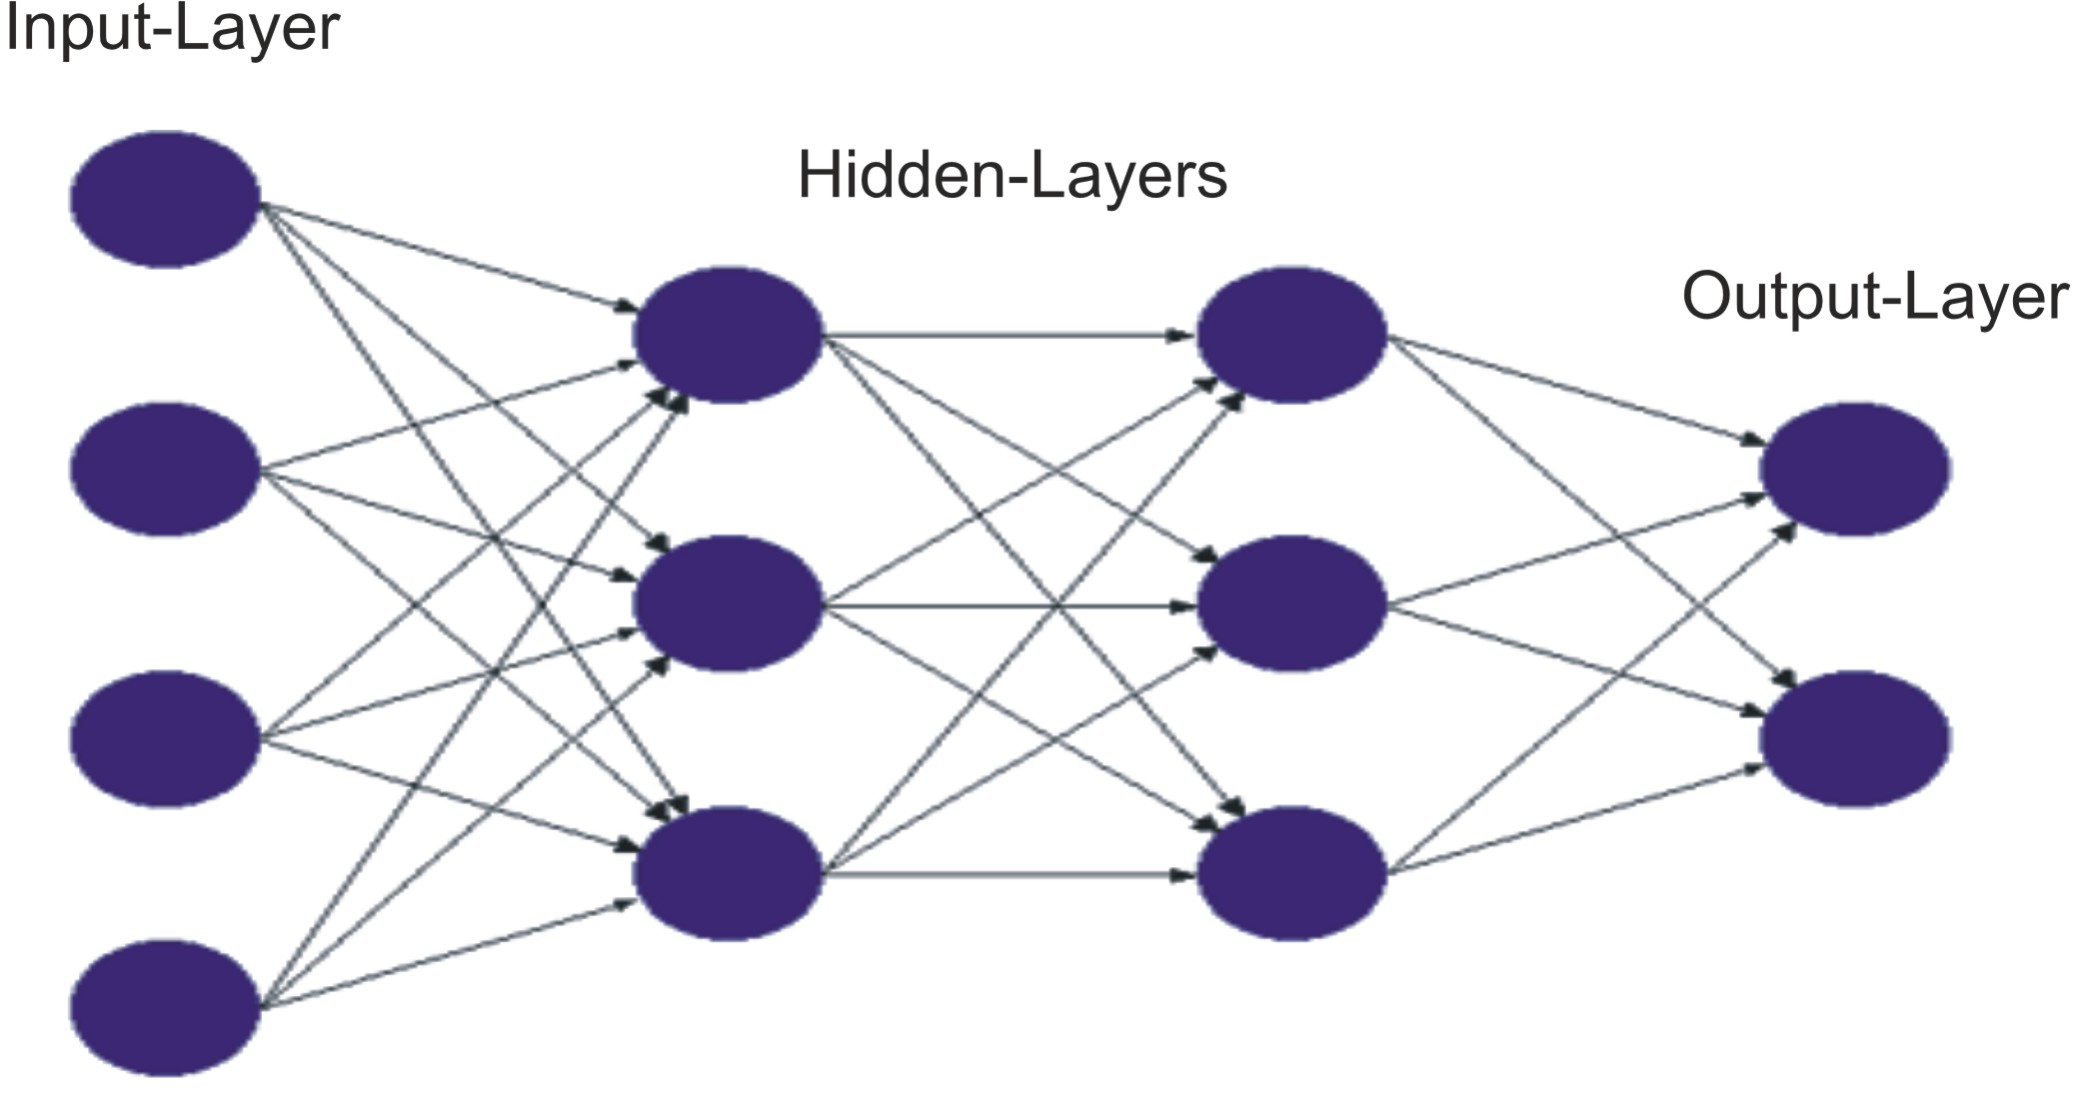
\includegraphics[scale=0.5]{Sources/nnet.png}
		\caption{Schematischer Aufbau eines künstlichen neuronalen Netzes \cite{bistra2018pic} }
	\label{img:KNN}
\end{figure}
\\
\\
Der Aufbau eines künstlichen neuronalen Netzes kann grundsätzlich in drei Schichten aufgeteilt werden (Abbildung \ref{img:KNN}). Die erste Schicht ist der \glqq Input Layer\grqq. Dieser \glqq Layer\grqq bekommt alle Eingangsdaten von einem beliebigen Datensatz. Jeder Pixel auf einem Bild wird mit einem Neuron verbunden, welche sich in der Gewichtung und dem Schwellwert unterscheiden können. Wird der Schwellwert überschritten, gibt das Neuron die verarbeiteten Informationen an die nächste Schicht weiter. Die zweite Schicht besteht aus einem oder mehreren \glqq Hidden Layer\grqq. Jeder \glqq Layer\grqq ist in dieser Schicht auf verschiedene Merkmale trainiert. Anfangs werden nur grobe Strukturen erkannt, wie beispielsweise Geraden oder Kanten. Diese Strukturen werden detaillierter, desto mehr \glqq Layer\grqq durchlaufen wurden. Die dritte Schicht besteht aus dem \glqq Output Layer\grqq. Die Muster die in den vorherigen Layern erkannt und zusammengesetzt wurden, vergleicht der \glqq Output Layer\grqq mit den trainierten Klassen und gibt eine prozentuale Wahrscheinlichkeit aus, welche Klassen in dem Bild enthalten sind.


  \subsection{Faltendes neuronales Netz}
Anders als bei einem KNN, welches auf Grundlage des menschlichen Gehirns entworfen wurde, orientiert sich ein \glqq Convolutional Neural Network\grqq (CNN) an dem Konzept des menschlichen Sehens \cite{lecun1989backpropagation}. Dabei werden maschinell kleine Bereiche visueller Informationen so simuliert, als wären sie benachbarte Sehnerven im Auge. Gerade für die Verarbeitung von Bilddaten werden häufig \glqq Convolutional Neural Networks\grqq eingesetzt \cite[326]{goodfellow2016deep}. Voraussetzung für die Verwendung eines CNN ist die matrixartige Anordnung der Datenpunkte, wie beispielsweise bei einem digitalen Bild.
\\
\\
Bei einem \glqq Convolutional Layer\grqq (Abbildung \ref{img:CNN}) wird über die Pixel des Eingabebildes eine Schablone gelegt. Die Schablone wird je nach Bildgröße mehrfach horizontal, wie auch vertikal verschoben \cite[327-335]{goodfellow2016deep}. Diese Layer haben meist eine ungerade quadratische Abmessung (3x3, 5x5, 7x7). Die frühen Schichten bilden zunächst ein Skalarprodukt der betroffenen Pixel und können dadurch grobe Kanten erkennen. Jeder Layer ist dabei auf eine bestimmte Art von Mustern trainiert. Je mehr Layer durchlaufen werden, desto genauer werden die Muster, welche das neuronale Netz erkennt.

\begin{figure}
    [h]
	\centering
	\includegraphics[scale=1.5]{Sources/cnn2.png}
		\caption{Funktionsweise eines Convolutional Neural Network\cite{info7040061}}
	\label{img:CNN}
\end{figure}

Der \glqq Pooling Layer\grqq oder auf deutsch, Vereinfachungsschicht (Abbildung \ref{img:CNN}) funktioniert ähnlich wie der \glqq Convolutional Layer\grqq \cite[336f.]{goodfellow2016deep}. Auch bei dieser Methode wird eine Schablone über die Pixel des Bildes gelegt und horizontal wie auch vertikal verschoben. Hierbei werden die Farbwerte der beteiligten Pixel verarbeitet. Es kann entweder der höchste Farbwert eines Pixels übernommen, oder der durchschnittliche Farbwert berechnet werden. Die letzten Schichten des Netzes bestehen aus dem \glqq Fully Connected Layer\grqq, welcher den normalen Aufbau eines künstlichen neuronalen Netzes darstellt \cite[14]{lecun1989backpropagation}. Das bedeutet alle Ausgaben werden, wie bei einem KNN, mit jedem Neuron verbunden. Die letzte Schicht übergibt seine Ausgaben an den Output Layer, welcher die Zuordnungswahrscheinlichkeiten der Objekte zu den trainierten Klassen berechnet.

\newpage

  \section{Durchführung}
In diesem Kapitel wird die praktische Durchführung beschrieben und gemachte Entscheidungen erläutert. Zu beginn werden die verwendeten Frameworks und die Entwicklungsumgebung vorgestellt. Da für das erstellen eines neuronalen Netzes eine hohe Anzahl an Trainingsdaten, sowie viel Rechenleistung benötigt wird, folgt eine Evaluation von vortrainierten Netzen welche für diese Projekt verwendet werden sollen. Im Anschluss werden die zu verwendenden Klassen und Trainingsdaten erstellt. Abschließend werden die ausgewählten Netze mit den generierten Trainingsdaten trainiert. \\
\\

\subsection{Entwicklungsumgebung}
Um ein bestehendes neuronales Netz neu zu trainieren werden neben dem Neuronalen Netz weitere Frameworks sowie eine Entwicklungsumgebung benötigt. In den kommenden Unterpunkten wird die Entwicklungsumgebung sowie alle benötigten Bibliotheken aufgeführt. 

  \subsubsection{Verwendete Hardware Konfiguration}
Das Netz wurde auf einem Windows 8.1 Betriebssystem trainiert. Berechnet wurden die Trainingsschritte von einer Nvidia GeForce GTX 980 GPU mit 4GB VRAM (Grafikspeicher), einer Intel Core i5 CPU und 16GB RAM (Arbeitsspeicher). Für einen Trainingsschritt, mit der verwendeten Konfiguration, benötigt die Grafikkarte durchschnittlich 250ms-600ms. Im Vergleich hat die CPU mit 2-6 Sekunden pro Schritt, ungefähr die Acht fache Zeit benötigt. Der Vorteil liegt hier eindeutig bei der Grafikkarte, durch die Optimierung in Matrixmultiplikationen und wird aus diesem Grund für das Training verwendet.

  \subsubsection{Anaconda python}
Die im späteren aufgeführten CNN's sowie die Tensorflow API wurden in der Programmiersprache Python erstellt, weswegen wir zum um-trainieren mit Python arbeiten. Des weiteren bietet Python eine Vielzahl an verfügbaren Bibliotheken welche wir benötigen. Anaconda \cite{conda2018} ist eine \glqq Open-Source-Distribution\grqq für die Programmiersprache Python. Mit dieser können wir gleichzeitig mehrere Versionen von Python generieren und die notwendigen Bibliotheken installieren. Anaconda bietet den Vorteil einfach zwischen den verschieden Python Versionen wechseln zu können \\
In diesem Projekt wurde mit der Python version 3.6.7 gearbeitet.

  \begin{itemize}
	\item Installation von Python 3.6.7: conda create -n <Name> python=3.6.7
  \end{itemize}
  
  \subsection{Frameworks}
Um ein künstliches neuronales Netz zu trainieren, wird ein Framework und mehrere Programm-Bibliotheken benötigt. Die Auswahl wird im folgenden aufgezählt und kurz erläutert.
 
  \subsubsection{Tensorflow}
Bei Tensorflow \cite{google2018tens} handelt es sich um eine Plattform unabhängige Programmbibliothek unter Open-Source-Lizenz, die sich für Aufgaben rund um maschinelles Lernen und Künstliche Intelligenz (KI) einsetzen lässt. Ursprünglich entwickelte Google die Software für den internen Bedarf. Das Framework bietet vielfältige Einsatzmöglichkeiten und gestattet es, lernende neuronale Netze zu erstellen und diese zu verändern. Es zeichnet sich durch seine gute Skalierbarkeit aus und ist auf unterschiedlichen Systemen vom Smartphone bis zu Clustern mit vielen Servern einsetzbar. Außerdem stellt Google verschiedene trainierte Modelle bereit welche für das Projekt verwendet können. Tensorflow kann auf allen CPU's betrieben werden, oder mit Nvidia Grafikkarten, welche CUDA unterstützen.

  \begin{itemize}
\item Installation in Python: pip install --upgrade gpu-tensorflow
  \end{itemize}
  
Verwendet wird zusätzlich die API von Tensorflow (Models) für die Objekterkennung. In dieser wird eine Grundstruktur für das Trainieren eines CNN zur Verfügung gestellt, welche man je nach Verwendungszweck anpassen kann.
  
  \subsubsection{Benötigte Bibliotheken}
Für das Arbeiten mit Tensorflow und CNN's benötigt man einige spezielle Python Bibliotheken. Diese werden im folgenden aufgeführt und erläutert. Die Installation geschieht hier über den \glqq Package Installer \glqq von Python.
\\
 
\textbf{Pillow}\\\\
Pillow ist eine \glqq Imaging Library \glqq für Python. Diese Bibliothek wird dafür genutzt um Bilddateien öffnen, verändern und speichern zu können.

  \begin{itemize}
\item Installation in Python: pip install --upgrade pillow
  \end{itemize}

\textbf{lxml}\\\\ 
lxml ist eine Weiterführung der XML Sprache für Python. lxml erweitert dabei den Elementebaum von XML stark. Verwendet wird lxml dafür, um die Markierungen von Objektsklassen und deren Positionen auszulesen. Durch die Arbeit mit Elementbäumen werden nur die benötigten Informationen herausgefiltert, woraus einem bessern Laufzeitverhalten resultiert.
  
  \begin{itemize}
\item Installation in Python: pip install --upgrade lxml
  \end{itemize}
  
  
\textbf{Cython}\\\\
Python ist im vergleich zu C eine recht langsame Programmiersprache, was die Ausführungzeit des Programmcodes wesentlich erhöht. Cython ist eine Programmbibliothek und auch Programmiersprache, welche die wesentlich langsame Programmiersprache Python erweitert und in der Ausführung beschleunigt. Dabei wird Python-Code in C kompiliert oder es kann externer code von C, eingebunden werden um ihn für die Ausführung zu nutzen. Das hat den Vorteil, das die Geschwindigkeit des Programms erhöht wird. Gerade für das Trainieren künstlicher neuronaler Netze, wird viel Rechenleistung benötigt.

  \begin{itemize}
\item Installation in Python: pip install --upgrade Cython
  \end{itemize}

\textbf{Jupyter}\\\\
Jupyter oder auch \glqq Jupyter Notebook\grqq ist eine open-source Web Applikation die es ermöglicht Dokumente welche Live Code, Abbildungen oder Text beinhalten zu teilen. Dabei können Inhalte von Dateien im Browser aufgerufen und ausfeführt werden. Verwendet wird diese Bibliothek um die korrekte installation von Tensorflow zu überprüfen.  

\begin{itemize}
\item Installation in Python: pip install --upgrade jupyter
  \end{itemize}
  
\textbf{matplotlib}\\\\
Die Programmbibliothek matplotlib ermöglicht es mathematische Formlen in der Python-Konsole oder im Code zu verarbeiten und zu visualisieren.
Matplotlib wird verwendet um die Erkennung von Objekten und deren Positionen auf einem Bild dazustellen.

  \begin{itemize}
\item Installation in Python: pip install --upgrade matplotlib
  \end{itemize}
  
\textbf{Pandas}\\\\
Pandas ist eine Programmbibliothek von Python. Der Name stammt von \glqq Paneldata\grqq, was eine Bezeichnung von Datensätzen ist. Diese Bibliothek ermöglicht eine enfache selektierung und Inditzierung von Daten. In diesem Projekt wird Pandas für die Erhebung von Informationen aus den Trainingsdaten verwendet und für die Generierung von Graphen.

  \begin{itemize}
\item Installation in Python: pip install --upgrade pandas
  \end{itemize}
  
\textbf{opencv-python}\\\\
OpenCV steht für \glqq Open Source Computer Vision Library\grqq  und ist eine freie Programmbibliothek für maschinelles Sehen. Diese Bibliothek ermöglicht die Aufteilung eines Bildes in verschiedene Bildbereiche. Außerdem können weitere Bildoptimierungen vorgenommen werden, wie das anpassen der Bild Helligkeit.

  \begin{itemize}
\item Installation in Python: pip install --upgrade opencv-python
  \end{itemize}

  \subsection{Abwägung von neuronalen Netzen} 
In der folgenden Abwägung werden einige verfügbare Netze aufgeführt, die für Tensorflow zur Verfügung gestellt werden. Dabei werden die aufgeführten Modelle in Genauigkeit und Geschwindigkeit verglichen.
 
  \subsubsection{Auswahl des Netzes} 
In Hinsicht auf Trainierte Netze bietet \glqq Tensorflow\grqq einige Möglichkeiten an. Hierbei handelt es sich um die \glqq Tensorflow detection model zoo\grqq \cite{google2018zoo} welche mit verschiedensten Datensätzen ausgiebig trainiert wurden. Bei dem COCO Datenset handelt es sich um \glqq Common Objects In Context\grqq \cite{common2018data} und beinhaltet rund 330 Tausend Bilder, welche über 1.5 Millionen schichten in 90 Klassen trainiert wurden. Da es sich um häufige auftretende Objekte in einer realen Umgebung handelt, sind die Modelle gut für unser vorhaben geeignet. In der folgenden Tabelle, wurden ein paar dieser Modelle ausgesucht und verglichen.
\\
\\

\begin{table}
[h]
\begin{tabular}{|l|c|c|c|}
 
Modell Name & Geschwindigkeit & COCO mAP & Ausgabe\\
 & & & \\
faster\_rcnn\_inception\_v2\_coco & 58 ms & 28 & Boxen\\
 & & & \\
faster\_rcnn\_resnet50\_coco & 89 ms & 30 & Boxen\\
 & & & \\
rfcn\_resnet101\_coco & 92 ms & 30 & Boxen\\
 & & & \\
faster\_rcnn\_resnet101\_coco & 106 ms & 32 & Boxen\\
 & & & \\
ssd\_mobilenet\_v1\_fpn\_coco & 53 ms & 32 & Boxen\\
 & & & \\
ssd\_resnet\_50\_fpn\_coco & 76 ms & 35 & Boxen

\vspace{0.5 cm}
 
\end{tabular}
\caption{Trainierte Modelle auf dem COCO Dataset \cite{google2018zoo}}
\end{table}


In der Tabelle, werden 6 mögliche Modelle aufgeführt wobei diese anhand der durchschnittlichen Geschwindigkeit, der Genauigkeit und eines Ausgabetyps verglichen werden. Die zweite Spalte, COCO mAP (mean average Persition) gibt die mittlere durchschnittliche Genauigkeit an, mit welcher es Objekte erkennt. Berechnet wird diese durch die Genauigkeit der richtigen Ergebnisse im Vergleich auf alle ausgeführten Trainings Durchläufe des Systems. Es stellt als keine Prozentuale Wahrscheinlichkeit dar. In der letzten Spalte wird die Ausgabeform beschrieben. Hierbei kann zwischen Boxen und Masken unterschieden werden. Dabei wird je nach Ausgabetyp entweder ein viereckiger Kasten (Abbildung \ref{img:Boxes}) um das object erstellt, oder es wird eine Maske (Abbildung \ref{img:Mask}) über dieses gezogen. In der Auswahl befinden sich jedoch keine Modelle welche eine Maskierung ausgeben.

%einbinden einer Grafik 
\begin{figure} 
	[h]
	\centering
    \subfigure[Makierung durch Maskierung \cite{artikle2018test2}]{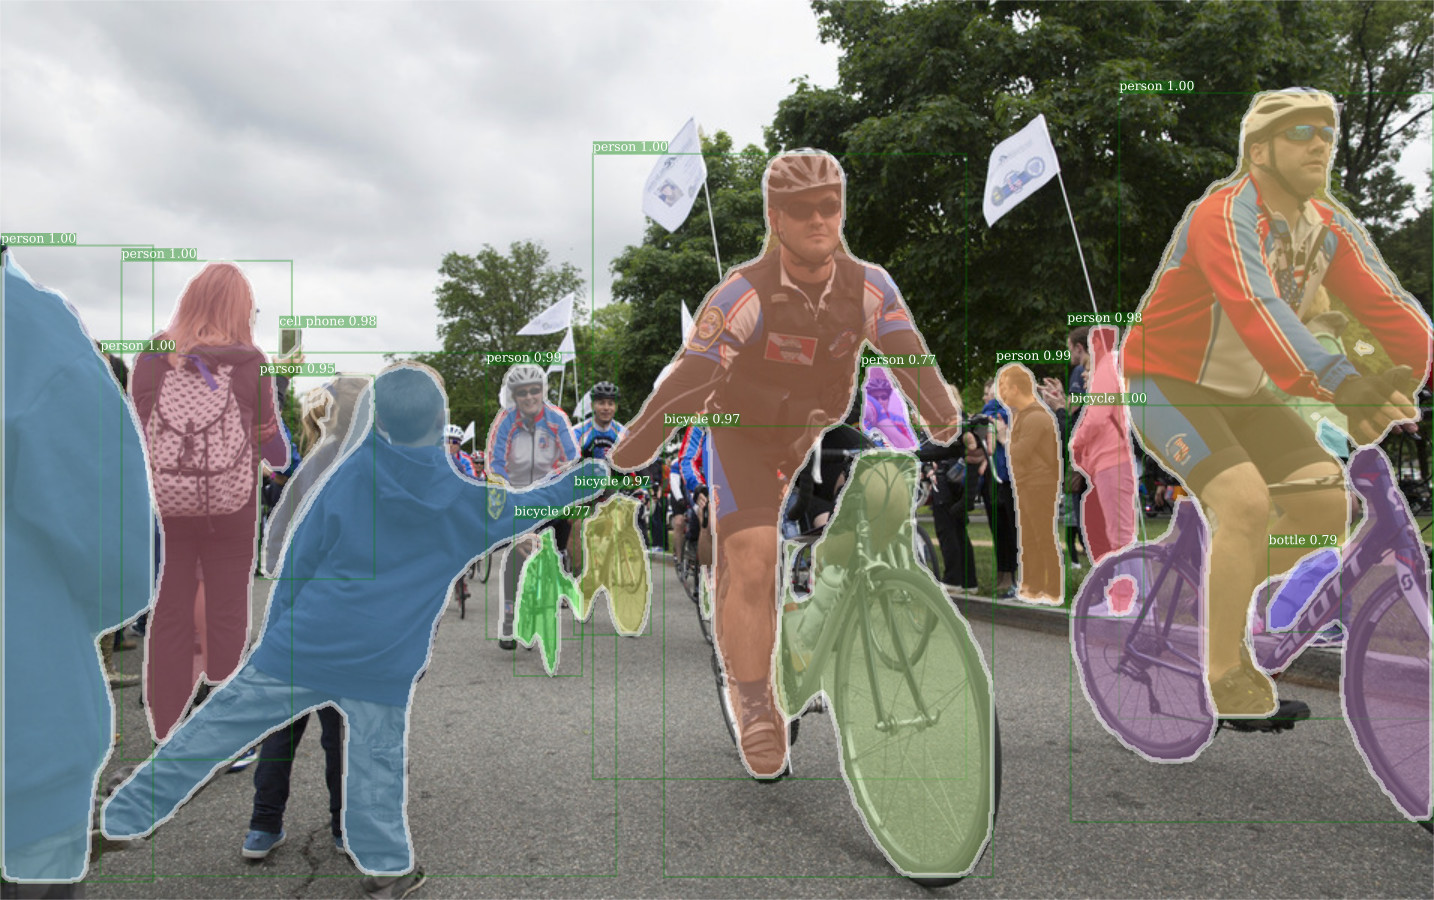
\includegraphics[width=0.39\textwidth]{Sources/sample.jpg}}
    \label{img:Mask} 
    \subfigure[Makierung durch Kästen \cite{google2018test1}]{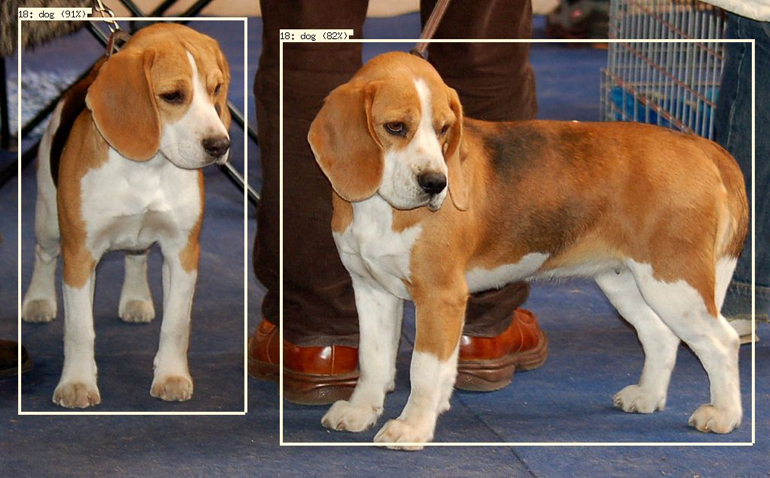
\includegraphics[width=0.39\textwidth]{Sources/boxes.jpg}}
    \label{img:Boxes} 
\caption{Ausgaben von Neuronalen Netzen} 
\end{figure} 

\newpage

Bei dem Vergleich der Modelle fällt auf, dass alle eine ähnliche Genauigkeit aufweisen und sich nur leicht unterscheiden. In der Geschwindigkeit jedoch werden die Unterschiede erkennbar größer. Durch die hohe Geschwindigkeit und vergleichsweise hohe Genauigkeit, wird vorerst das faster\_rcnn\_inception\_v2\_coco Modell getestet, und ausgewertet.
\\

Das ausgewählte Modell wurde mit 6 Klassen um-trainiert. Die Klassen bestanden aus einem Skart-kartenset von Neun bis Ass \cite{evan2018pic}. Rund Fünf Stunden wurde das Netz trainiert, und hat dabei 60 tausend Testdurchläufe absolviert. Eine Überprüfung des Netzes hat eine Genauigkeit von 97 bis 99 Prozent ergeben. Auch Tests ergeben das die Erkennung fehlerfrei funktioniert. Das Testbild (Abbildung \ref{img:Kartenset} zeigt, das alle Karten mit einer hohen Wahrscheinlichkeit identifiziert werden konnten.
\\
\begin{figure}
    [h]
	\centering
	\includegraphics[scale=0.5]{Sources/kartenset.png}
	\caption{Analysiertes Bild, durch das Testnetz}
	\label{img:Kartenset}
\end{figure}
\\
Das erfolgreiche Training und testen des Netzes hat die Verwendung des Ausgewählten Modells bestärkt. Die Vorgehensweise sieht in den weiteren Schritten eine Definition und Festlegung der Trainings-Daten für das benötigte neuronale Netz. 

  
  \subsection{Trainingsdaten Generieren} 
Zu beginn hat ein untrainiertes neuronales Netz, in seinen Neuronen, zufällige Gewichtungen und Schwellwerte, da es bis zu diesem Zeitpunkt noch keine Informationen darüber hat, welche Objekte es erkennen soll und welche Eigenschaften diese haben. Damit das zu entwickelnde neuronale Netz die Informationen erhält welche für eine Klassifizierung notwendig sind müssen zunächst Trainings und Testdaten generiert werden. Für das Training werden optimaler weise mehrere Tausend Trainings- und Testbilder benötigt, damit eine möglichst hohe Genauigkeit erreicht werden kann. Auch die Trainingsphase dauert in der Ausführung einige Stunden. 
\\
\\
Wie bereits in vorherigen Kapitel beschrieben wird wegen der begrenzten Zeitressource ein vortrainiertes Netz verwendet welches mit den COCO Testdaten trainiert wurde verwendet. Der Vorteil eines vortrainierten Netzes besteht darin, das die Gewichtungen der frühen Schichten gut eingestellt sind und diese nicht verändert werden müssen. Lediglich die letzten Schichten sollen mit den eigenen Daten umtrainiert werden. Durch die guten Einstellungen der ersten Schichten, werden weniger Trainings- und Testdaten benötigt, um eine hohe Genauigkeit des Neuronalen Netzes zu erreichen.

  \subsubsection{Funktionsweise}
Bei einem untrainierten Netz werden jedem Neuron zunächst ein zufälliges Anfangs-Gewicht sowie ein Schwellwert zugewiesen. Beim starten der Trainingsphase werden Daten in das Netz eingeführt. Jedes Neuron verarbeiten nun alle Eingangssignale mit der zugewiesenen Gewichtung und geben die Ergebnisse an das nächste Neuron weiter. 
\\
\\
Im Output-Layer wird nun das Ergebnis der Berechnungen ermittelt. Das Ergebnis des Netzes wird mit der Tatsächlichen Bezeichnung des Objektes verglichen. Lag das Netz bei der Bestimmung falsch wird zunächst der entstandene Fehler Berechnet und die Neuronen werden dementsprechend angepasst. Dabei werden die Gewichtungen der Neuronen so stark verändert je mehr Einfluss diese auf das resultierende Ergebnis hatten. Dieser Vorgang wird nun viele male wiederholt. \\
  
  \subsubsection{Auswahl der Klassen} 
Bei der Auswahl der Klassen wurde darauf geachtet, die Genauigkeit des Netzes zu erkennen, indem Klassen ausgewählt werden, welche Ähnlichkeiten aufweisen jedoch ????????????????? unterschiedliche Bezeichnungen haben??????????. Beispiele sind hier Flaschen, Tetra Packs oder auch Schachteln.

\vspace{0.5 cm}

\begin{itemize}

\item ID: 1 Name: \glqq Milch, Packung\grqq

\item ID: 2 Name: \glqq Orangensaft, Packung\grqq

\item ID: 3 Name: \glqq Wasser, Flasche\grqq

\item ID: 4 Name: \glqq Bier, Flasche\grqq

\item ID: 5 Name: \glqq Brunch, Aufstrich\grqq

\item ID: 6 Name: \glqq Margarine, Aufstrich\grqq

\end{itemize}
  

Damit das zu entwickelnde Netz für die ausgewählten Klassen verwendet werden kann, muss ein großer Datensatz generiert werden. Um Aussagen über die Genauigkeit des Netzes machen zu können wurden Objekte mit hoher Ähnlichkeit verwendet. Als Testobjekte wurden zwei Tetra Packs, zwei Flaschen und zwei Aufstriche verwendet. Die Einteilung der Klassen ist in der folgenden Tabelle aufgeführt.
\\
\\

\begin{table}
[h]
\centering
\caption{Ausgewählte Klassen und Struktur}
\label{klassen}
\begin{tabular}{|c|l|c|}
  
    Klasse   &   Bezeichnung   &   Bereich   \\
  & & \\
    1   &   Milch - Packung   &   1-99   \\
  & & \\
    2   &   Orangensaft - Packung   &   100-199   \\
  & & \\
    3   &   Wasser - Flasche   &   200-299   \\
  & & \\
    4   &   Bier - Flasche   &   300-399   \\
  & & \\
    5   &   Brunch - Aufstrich   &   400-499   \\
  & & \\
    6   &   Margarine   &   500-599   \\
  & & \\
    7   &   Gemischt   &   600-699
  
\end{tabular}
\end{table}

\vspace{1 cm}

Zunächst müssen Testdaten in Form von Bildern generiert werden, wozu Bilder aus dem Internet, sowie selst erstellte Fotografien der Objekte verwendet, welche aus  verschieden Winkeln und unterschiedlichen Lichtverhältnissen aufgenommen wurden. Dabei sollte ein Bild die Größe von 200 KB nicht übersteigen, damit das Training erfolgreich verläuft und nicht unnötig viel Zeit benötigt. Die selbst erstellten Bilder wurden deshalb um den Faktor 0.2 verkleinert. Verwendet wurde für die Komprimierung das in Python geschriebenes Programm (reziser.py).\\
\\
Zum erstellen eines Ground True müssen die Bilder gelabelt werden, hierfür wurde das Programm labelImg.py verwendet. Beim labeln werden die zu klassifiezierenden Objekte auf dem Bild mit den Positionsdaten und Bezeichnung markiert und in einer XML Datei abgespeichert. Nach dem markieren werden die Daten in Trainings und Testdaten aufgeteilt. 80 Prozent kommen in den Trainingsordner und 20 Prozent in den Testordner. Für die Durchführung des Trainings werden die Informationen der einzelnen XML Dateien, in zwei CSV Dateien zusammengefasst. Diese Dateien beinhalten Tabellen in denen alle notwendigen Informationen zu den Bildern aufgeführt werden. Verwendet wird dafür das Programm xml\_to\_csv.py.\\
\\

  
  \subsection{Trainieren}
Nachdem alle Bilddaten gelabelt wurden und die CSV Dateien für die Trainings- und Testdaten erstellt wurden, kann das Training beginnen. Zusätzlich zu den Traningsdaten wird eine Labelmap (labelmap.pbtxt) benötigt in welcher die aus Kaptitel 3.4.2 ???? Kapitel nummer Prüfen ansonsten Kapitel überschrieften oder querwerweise verwenden ????ausgewählten Klassen aufgeführt werden. Außerdem wird die Konfigurationsdatei des verwendeten Netzes (faster\_rcnn\_inception\_v2\_coco) benötigt. Das Training wird mit Ausführung des training.py Programms gestartet. Ab diesem Zeitpunkt, benötigt das Training viel Zeit.\\\\
Zusätzlich Parameter: \\
\textbf{--logtostderr}\\
\textbf{--train\_dir=training/}\\
Dieser Parameter gibt den Pfad zum Ordner an in welchem die Trainingsergebnisse Gespeichert werden sollen.\\
\textbf{--pipeline\_config\_path=training/faster\_rcnn\_inception\_v2\_coco.config}\\
Dieser Parameter gibt den Pfad zu der KOnfigurationsdatei an\\\\
\\
Damit die Ergebnisse so gut wie möglich ausfallen, wird das Netz ca. 10 Stunden, mit der in Kapitel????????????? beschriebenen Konfiguration trainiert. IN dieser Zeit wurden 200.000 Trainings- und Testdurchläufe ??? Was ist der unterscheid zwischen trainig und Test durchläufen / Ist das TEsten nict teil des Trainings????   durchgeführt. Kurz vor dem Abschluss der Trainingsphase wird ein durchschnittlicher \glqq loss\grqq von 0,03 erreicht. ?????????? der begriff loss ist noch nicht eingeführt?????????????? Alle fünf minuten kann mit hilfe des export\_inference\_graph.py programms ein sogenannter \glqq frozen inference graph\grqq ?????????? einmal kein geschrieben und einmal groß ?????????? generiert werde,n welcher unser Künstliches neuronales Netz darstellt.\\\\
Mitgegebenen Parameter:\\
\textbf{--input\_type image\_tensor}\\
\textbf{--pipeline\_config\_path legacy/training/faster\_rcnn\_inception\_v2\_coco.config}\\
Gibt den Pfad zur config Datei an.\\
\textbf{--trained\_checkpoint\_prefix legacy/training/model.ckpt-XXXX}\\
Gibt den Pfad zur letzten Speicherstand des Trainings an.\\
\textbf{--output\_directory inference\_graph}\\
Bestimmt den Ort an welchen der Graph exportiert wird.\\\\

Nach Erstellung des \glqq Frozen Inference Graph\grqq ?????????? einmal kein geschrieben und einmal groß ??????????, welcher die Gewichtingen und Objektklassen enthält, ist das Netz an sich fertig und bereit für den praktischen Test. Dafür wurde aus der object\_detection\_tutorial.ipynb Datei von der Tensorflow API ein ausführbares Programm für die Testzwecke geschrieben. Im weiteren wird der Testverlauf beschrieben und Ausgewertet.
  
\newpage

\section{Testergebnisse}
In diesem Kapitel soll die Zuverlässigkeit und die Geschwindigkeit des neuronalen Netzes geprüft und ausgewertet werden. Dazu wird das Netz mit nicht markierten und dem Nertz unbekannten Bildern getestet. Es soll sichergestellt werden, dass das Netz die Objekte nicht bereits durch das Training kennt. Anschließend wird überprüft wie zuverlässig das Netz ist ??? Was meisnt du mit zuverlässig / robust gegebüber falsche klassifizierung , falsch detektionen  ???? und ob es alle Objekte erkannt wurden. 
\\
Tensorflow bietet mit dem Tool Tensorboard die Möglichkeit den fortschritt des Trainings grafisch darzustellen. In der folgenden Grafik wird der auftretende \glqq Loss \glqq in Verhältnis zu der Trainingszeit gestellt. 
\\
 \begin{itemize}
\item tensorboard --logdir=legacy/training --host=127.0.0.1
  \end{itemize}
  
\begin{figure}
    [h]
	\centering
	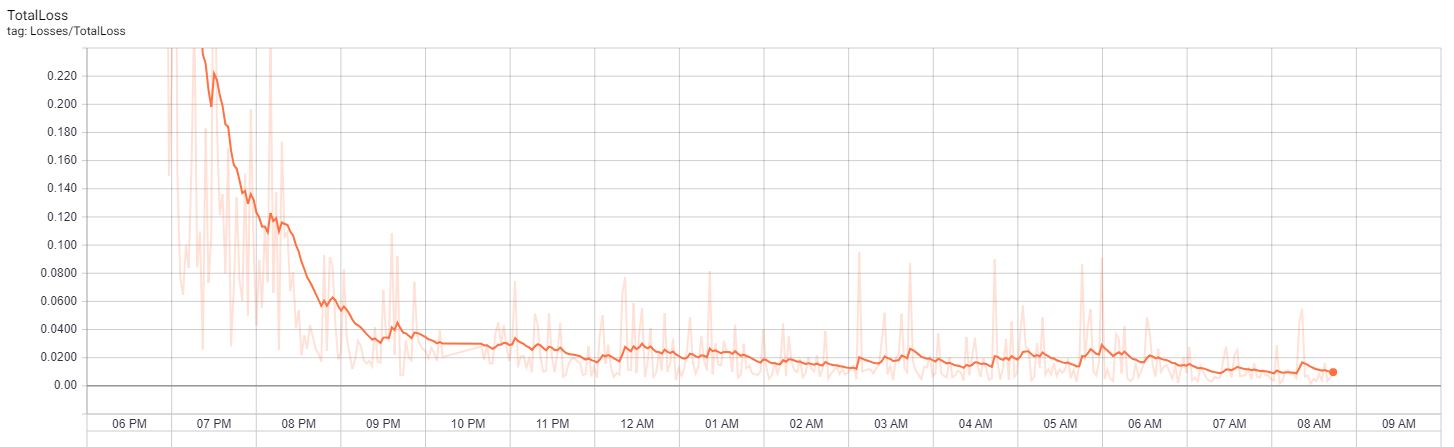
\includegraphics[scale=0.4]{Sources/loss_graph_200000.jpg}
	\caption{Loss Graph des umtrainierten inceptionV2}
	\label{img:loss_graph_200000}
\end{figure}

Der \glqq Loss\grqq stellt dabei keine Prozentangabe dar, sondern ist eine Zusammenfassung der Fehler, die für jedes Beispiel in Trainings- oder Validierungssätzen gemacht wurden. Je kleiner der \glqq Loss\grqq dabei ist, desto höher ist die Wahrscheinlichkeit ????das die Klassifizierung richtig ist ??? . Um die Grafik zu veranschaulichen, wurden kurzfristige Schwankungen geglättet. Innerhalb der ersten 4 Stunden des Trainings den größten fortschritt beobachtet werden. In dieser Zeit, ist der \glqq Loss\grqq von anfänglich 2.0 auf 0.05 gesunken. Dabei wurden rund 60.000 Trainingseinheiten durchlaufen.\\
Bei den ersten Testergebnissen welche in Abbildung ????????????? zu sehen sind konnten alle Objekte erkannt und ihnen eine Klasse zugewiesen werden. Jedoch wurde die \glqq Orangensaft - Packung\grqq mit hoher Wahrscheinlichkeit als \glqq Milch - Packung\grqq falsch klassifiziert. Was auf die hohe Ähnlichkeit der Objekte zurückzuführen ist.
\\

\begin{figure}
    [h]
	\centering
	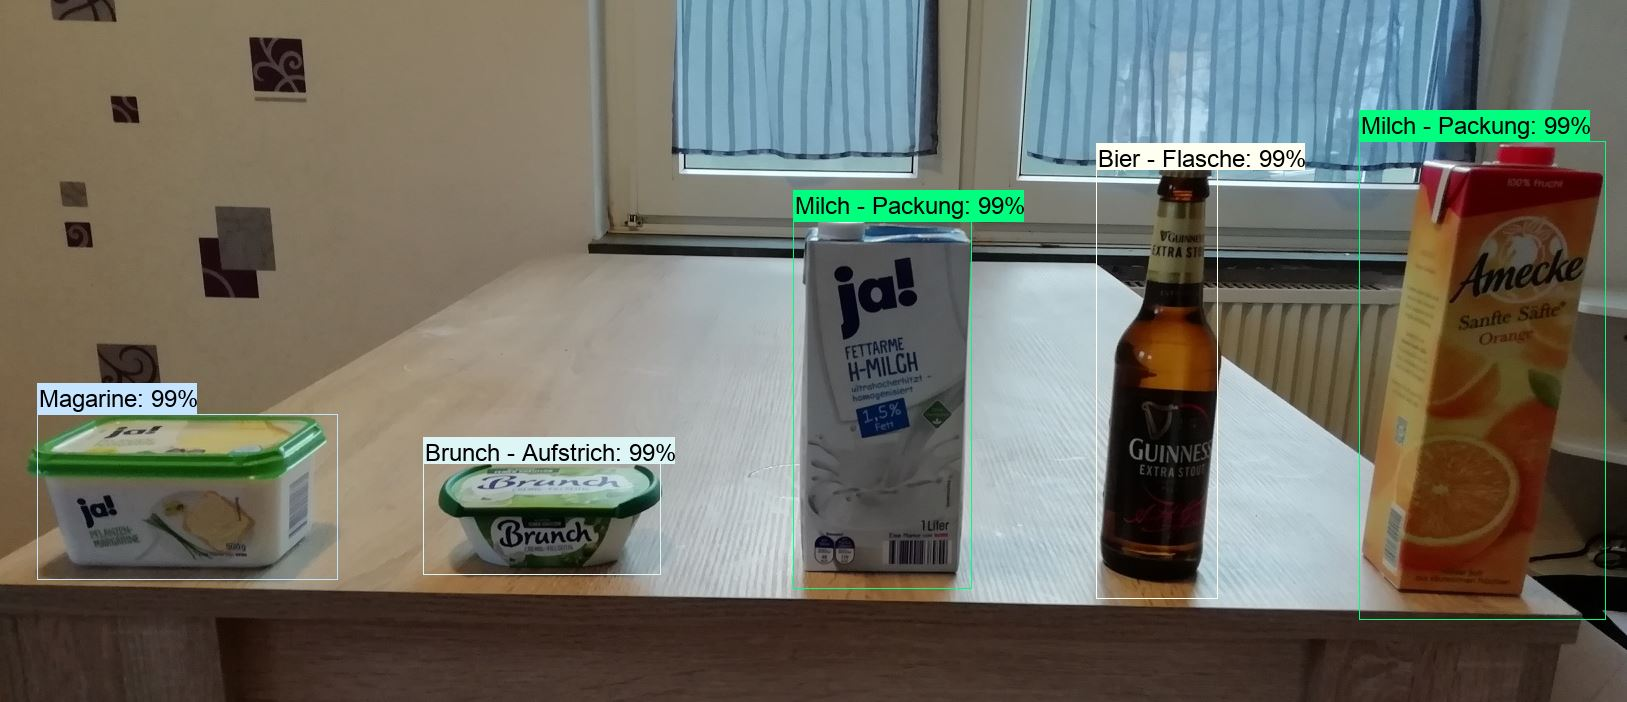
\includegraphics[scale=0.3]{Sources/Erster_Test.jpg}
	\caption{Erster Test des neuronalen Netzes}
	\label{img:TestNN}
\end{figure}

Aufgrund der falschen Klassifizierung wurde ein weiteres vortrainiertes Netze mit dem generierten Datensatz trainiert und getestet. Das dafür ausgewählte Netz ist das faster\_rcnn\_resnet101\_coco. Dieses Modelle wurden aus der Tabelle? ausgewählt, da die mittlere durchschnittliche Genauigkeit.
\\
\\
Das zweite Modell welches trainiert wurde ist das faster\_rcnn\_resnet101\_coco mit einer mAP ????mAP nicht eingrführter begriff????????? von 32 dafür ist es aber auch wesentlich langsamer. Für einen Trainingsdurchlauf benötigt das Modell mit rund 600ms im durchschnitt, mehr als doppelt so lange wie das faster\_rcnn\_inception\_v2\_coco. Es benötigt dafür aber auch nur die Hälfte an Durchläufen, um eine ähnlich niedrigen 'Loss' zu erreichen.\\ 

\begin{figure}
    [h]
	\centering
	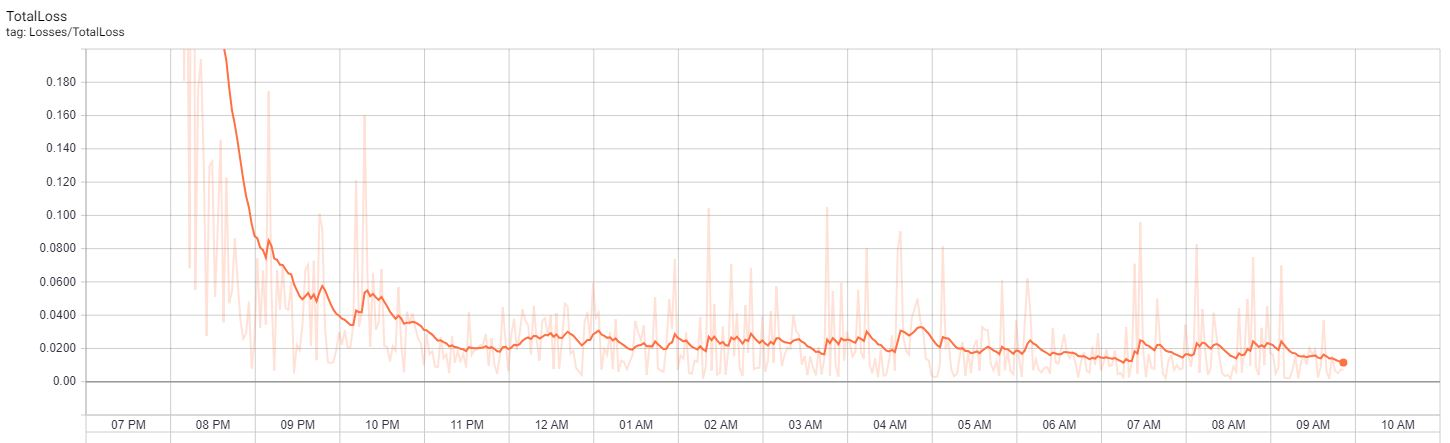
\includegraphics[scale=0.4]{Sources/loss_graph_resnet101.jpg}
	\vspace{0.5 cm}
	\caption{Loss Graph des umtrainierten resnet101}
	\label{img:loss_graph_resnet101}
\end{figure}

Die Testergebnisse der einzelnen Klassen zeigen das die erreichte Genauigkeit besser ist, so das allen erkannten Objekten die richtigen Klassen zugewiesen wurden. Dieses Netz ist zeigte sich aber deutlich Störungsanfälliger so dass je nach Winkel nicht immer alle Objekte erkannt wurden. Um die Stabilität zu erhöhen, wurden die Trainingsdaten erweitert und das letzte Modell welches die höchste \glqq mAP\grqq hat auf den Datensatz trainiert????? Verstehe den Satz nicht :)  ?????.\\
\\
Weitere Test mit dem Netz haben ergeben, das die Erkennung der Orangensaft Packung funktioniert, solange das Bild und die Oberflächen der Objekte nicht zu dunkel werden. Das Bild (Bild) zeigt alle Trainierten Objekte mit welchen das Modell faster\_rcnn\_resnet101\_coco trainiert wurde. Hier kann man erkennen das alle Klassen richtig zugeordnet werden konnten.

\begin{figure}
    [h]
	\centering
	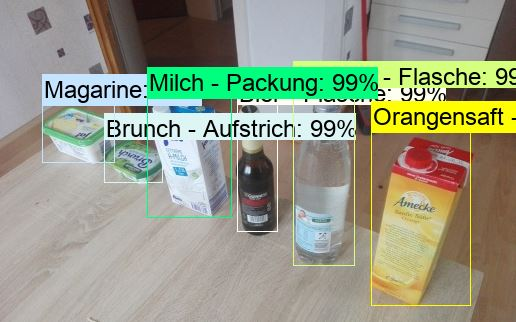
\includegraphics[scale=0.5]{Sources/final_detection.jpg}
	\vspace{0.3 cm}
	\caption{Objekt erkennung des optimierten resnet101}
	\label{img:loss_graph_resnet101}
\end{figure}

\\Im nächsten Kapitel sollen die Ergebnisse des Projektes, mit den Anforderungen verglichen und ausgewertet werden.


\newpage

\section{Fazit}
Abgesehen von den leichten schwächen in der Erkennung ähnlicher Objekte hat das generieren eines neuronalen Netzes Funktioniert. Schlechte Lichtverhältnisse haben die Ausgabe außerdem negativ beeinflusst. Lediglich bei ähnlichen Objekten, mit nur kleinen unterschieden, gab es Probleme mit der richtigen Identifizierung. Um ein finales Fazit geben zu können soll in diesem Kapitel auf die Anforderungen eingegangen werden, welche zu Beginn des Projektes festgelegt wurden.\\

\subsection{Bewertung durch Anforderungen}

Die ersten Zwei funktionalen Anforderungen konnten erfüllt werden. Lediglich die Genauigkeit konnte zunächst nicht zu voller Zufriedenheit erfüllt werden. Die meisten Objekte können bei schlechteren Bild- und Lichtverhältnissen erkannt werden, lediglich bei zu ähnlichen Objekten kann die Erkennung fehlerhaft sein, wie man bei der Milch und dem Orangensaft beobachten kann. Mit mehreren Trainingsdaten und einer Licht Korrektur könnte dies allerdings verbessert werden.\\
\\
Die organisationalen Anforderungen konnten auch zum Großteil erfüllt werden. Klassen können unkompliziert erweitert werden, indem Testdaten der gewünschten Klasse Generiert und gelabelt werden. Das trainieren und ausführen des Neuronalen Netzes ist zwar im Moment nicht mit einer Datei ausführbar, aber die notwendigen schritte sind nicht aufwendig. Die Installation aller Notwendigen Module und Bibliotheken kann durch die Eingabeaufforderung oder der \glqq shell\grqq ausgeführt werden. Lediglich für Anaconda muss man eine manuelle Installation durchführen. Das Netz kann auf jedem Endgerät mit der benötigten Entwicklungsumgebung betrieben werden. Für mobile Endgeräte ist das Netz jedoch wegen der benötigten Rechenleistung nicht geeignet.\\
\\
Bei den qualitativen Anforderungen kann man nicht jede erfüllen, weil je höher die Genauigkeit des Netzes ist, desto länger benötigt es um ein Bild auszuwerten. Umgekehrt sinkt die Genauigkeit umso schnelle das Netz arbeitet. Es wurde also darauf geachtet das es bei beiden Punkten solide Ergebnisse erzielt. Der Schwerpunkt lag aber auf der Genauigkeit des Netzes. Leicht verdeckte Objekte können auch bis zu einem Gewissen Punkt erkannt und richtig zugeordnet werden. Die Genauigkeit kann beispielsweise, durch mehrere Trainingsdaten erhöht werden.\\

\subsection{Bewertung der Netze}
Das Neuronale Netz funktioniert größtenteils wie gewollt, nur bei zwei Klassen kann nicht immer Korrekt unterschieden werden. Das liegt hauptsächlich an der hohen Ähnlichkeit der zwei Objekte. Die Genauigkeit könnte durch eine höhere Anzahl an Trainings und Testdaten verbessert werden. Außerdem könnte eine Angleichung der Lichtverhältnisse per Bildverarbeitung dafür sorgen, dass die Genauigkeit des Netzes steigt. Zwischen den getesteten Modellen wurde festgestellt, das die Übereinstimmung der Objekte einen wesentlichen unterschied in der Genauigkeit aufweisen, sodass eine etwas höhere Antwortzeit für den Verwendungszweck kein großes Problem darstellt.\\
\\
Abschließend, kann das Projekt als Erfolgreich angesehen werden, mit kleinen Optimierungen.

\newpage

\section{Aussicht}
Die Entwicklung eines neuronalen Netzwerkes hat gezeigt, das es Möglich ist den Inhalt Regal-Systeme mit Hilfe von Objekterkennung zu Identifizieren. Dabei ist aber auch aufgefallen, das mehr Trainingdaten benötigt werden je Ähnlicher sich die Klassen sind. Das bedeutet das für das geplante System eine große Anzahl an Trainingsdaten generiert werden müssen. Grundsätzlich ist es aber möglich mit den Ergebnissen weiter Arbeiten zu können.\\
\\
Für das Geplante System wären bis auf die Optimierung des Künstlichen neuronalen Netzes, die Systemschnittstellen welche zum einen das Bild vom Regal aufnimmt, verarbeitet und an das neuronale Netz weiter leitet und zum anderen müssen die Informationen der Bilderkennung an eine Datenbank übergeben werden, welche den Inhalt des Regals speichert. Darüber hinaus müsste eine Anwendung entwickelt werden, mit welcher der Benutzer den Inhalt des Regals managen kann.\\
\\
Die Optimierung soll aber Für die Nächsten Schritte im Vordergrund stehen. Für die anstehende Bachelorarbeit, soll die Verbesserung des Neuronalen Netzes im Vordergrund stehen. dabei gibt es drei wichtige Punkte welche behandelt werden müssen. Zum einen soll die Genauigkeit der Identifizierung bei ähnlichen Objekten erhöht werden. Außerdem sollen Bildaufnahmen so verarbeitet werden, das Lichtverhältnisse gleich sind oder eine Veränderung dieser Keinen Einfluss auf die Ergebnisse haben. Zusätzlich soll die Auswirkung schlechter Bildverhältnisse ermittelt und Verbessert werden.
   
\newpage

\printbibliography
  
\end{document}

